\section{Introduction}

The pursuit of Artificial General Intelligence (AGI) increasingly centers on agents: autonomous systems that can plan, reason, and act across diverse real-world tasks. Unlike conventional large language models (LLMs), which excel primarily at text generation, agentic systems must integrate reasoning with external actions, leverage memory across interactions, and adapt dynamically to unforeseen contexts. This shift positions LLM-based agents not just as conversational tools, but as general-purpose assistants capable of problem solving in open-ended, multi-modal, and continuously evolving environments.

Over the past two years, a wide range of agent frameworks have emerged. Early role-based multi-agent systems such as CAMEL~\cite{li2023camel} and MetaGPT~\cite{hong2024metagpt} demonstrated that structured collaboration could elicit disciplined reasoning behaviors, while more recent initiatives like OAgents~\cite{oagent}, AWorld~\cite{aworld2025}, Alita~\cite{qiu2025alita}, and OWL~\cite{owl2025} highlight new design philosophies: empirical scaling studies, co-evolutionary training loops, meta-tool creation, and modular planners. Benchmarks such as \gaia{}~\cite{mialon2023gaia} have revealed both the promise and the limitations of these systems—while they achieve notable progress, many approaches remain brittle, either due to over-reliance on hand-crafted workflows or lack of stability under real-world uncertainty.

\label{sec:intro}

\begin{figure}[t]
    \centering
    % \begin{subfigure}{0.8\linewidth}
    %     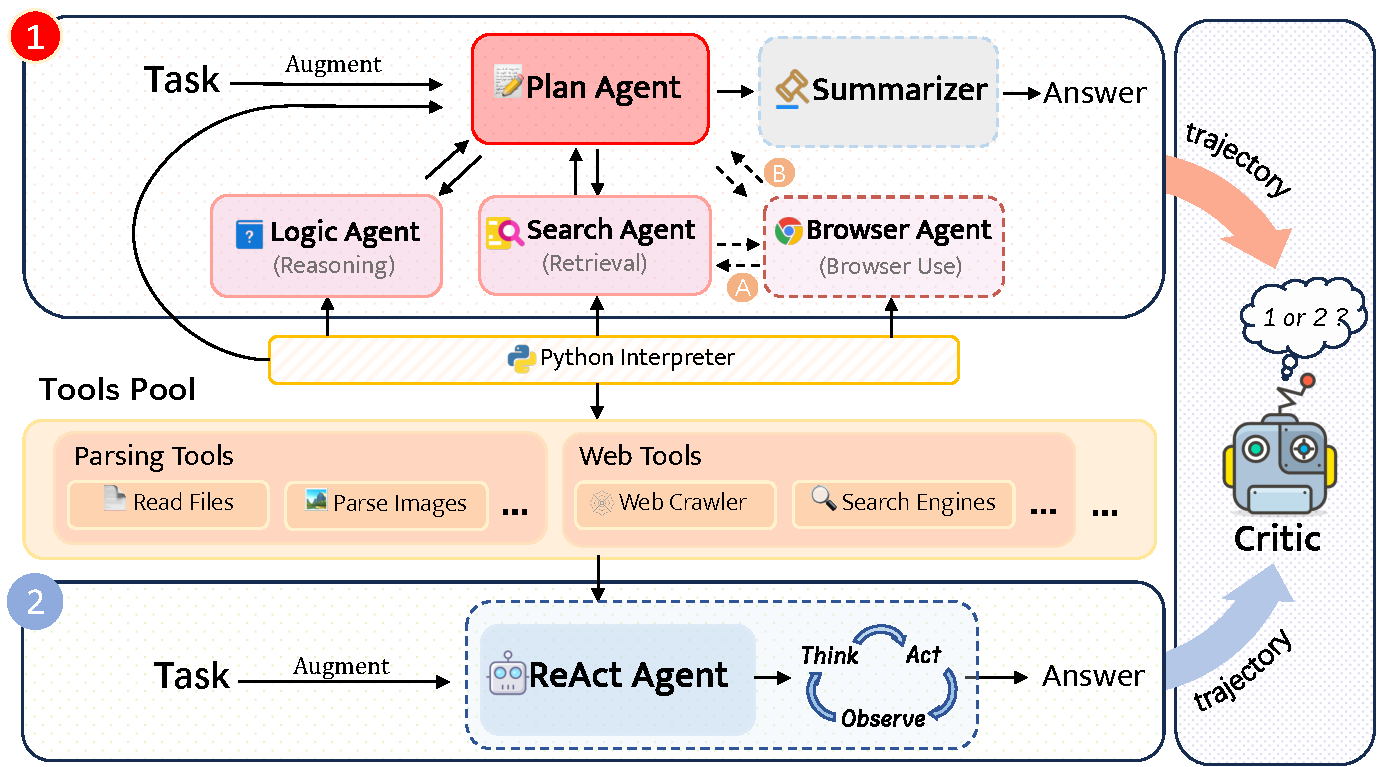
\includegraphics[width=\linewidth]{figs/overview.pdf}
    %     \caption{The fusion agent architecture.}
    %     \label{fig:overview}
    % \end{subfigure}\hfill
    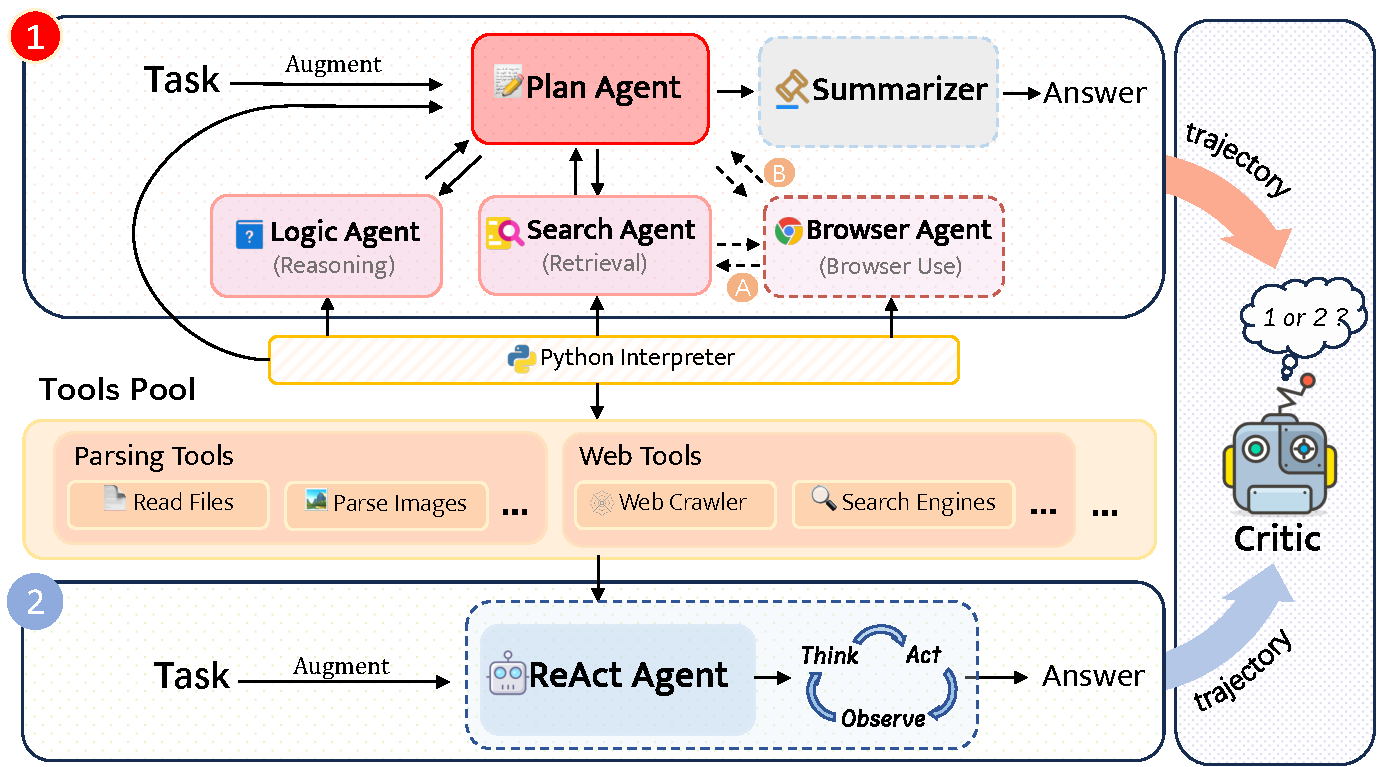
\includegraphics[width=0.8\linewidth]{figs/overview.pdf}
    \caption{The overview of the fusion agent architecture.}
    \label{fig:overview}
\end{figure}

In this work, we address these challenges by proposing a system-level framework that integrates three core components: (i) a heterogeneous ensemble of agents spanning both \texttt{Plan–Execute} and \texttt{ReAct} paradigms, coordinated through posterior voting to balance reliability and adaptability; (ii) a hierarchical memory design that combines working, semantic, and procedural layers to enable long-horizon continuity and adaptive control; and (iii) a refined tool ecosystem emphasizing search, code execution, and multimodal parsing, each wrapped into schema-consistent and auditable interfaces. Together, these design choices yield robust performance gains on the GAIA benchmark, setting state-of-the-art results among open-source systems and narrowing the gap to proprietary frameworks.
